\chapter{Mixed Side C\# (MiCS) Manual}
\label{chap:mics_manual}
TODO: Introduce what MiCS is used for in a single sentenc.
This chapter demonstrates how to use MiCS. The manual will illustrate how to write server side code that can be reused on client side in a safe manner. It is assumed that the developer uses Visual Studio and .NET 4.0. In this manual a simple registration form, shown in figure \ref{fig:manual_registrationform}, is created. The code is explained step-by-step but can also be found in its entirety in Appendix X.

% Todo: Insert appendix

\begin{figure}[H]
	\begin{center}
		\centerline{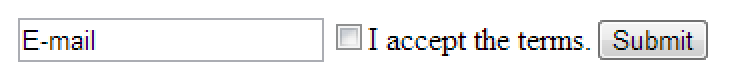
\includegraphics[width=12cm]{resources/images/manual_registrationform.png}}
	\end{center}
	\caption{Simple e-mail registration form.}
	\label{fig:manual_registrationform}
\end{figure}


\subsubsection{1. MiCS-enable Your Web Application} % (fold)
\label{ssub:mics_enable_your_web_application}
Create a new ASP.NET Web Application and goto the \texttt{Default.aspx.cs} Code Behind file. Remember to reference to MiCS.dll. Add using statements for \texttt{System.Html}, which contains all the ClientSide DOM types and \texttt{MiCS}. Change the \texttt{Default} class to inherit from \texttt{MiCSPage} instead of \texttt{System.Web.UI.Page}. See figure \ref{fig:mics_enable_web_application}.
\begin{figure}[H]
\begin{lstlisting}[language=CSharp,classoffset=1,morekeywords={Default,MiCSPage,Button,CheckBox,TextBox,EventArgs,ClientSide,InputElement,Document,CheckBoxElement,Window,MixedSide,Regex}]
...
using MiCS;
using System.Html;

namespace MiCSManual
{
    public partial class Default : MiCSPage
    {
        protected void Page_Load(object sender, EventArgs e)
        {
   
        }
    }
}
\end{lstlisting}
\caption{}
\label{fig:mics_enable_web_application}
\end{figure}
% subsubsection mics_enable_your_web_application (end)

Add the relevant controls to the page, as shown in figure \ref{fig:mics_add_controls}

\begin{figure}[H]
\begin{lstlisting}[language=CSharp,classoffset=1,morekeywords={Default,MiCSPage,Button,CheckBox,TextBox,EventArgs,ClientSide,InputElement,Document,CheckBoxElement,Window,MixedSide,Regex}]
...

public partial class Default : MiCSPage
{
  Button button;
  CheckBox checkBox;
  TextBox emailBox;

  protected void Page_Load(object sender, EventArgs e)
  {
    emailBox = new TextBox() { ID = "EmailBox", Text = "E-mail" };
    checkBox = new CheckBox() { ID = "CheckBox", Text = "I accept the terms."};
    button = new Button() { Text = "Submit" };

    form1.Controls.Add(emailBox);
    form1.Controls.Add(checkBox);
    form1.Controls.Add(button);
  }
}

...
\end{lstlisting}
\caption{Todo}
\label{fig:mics_add_controls}
\end{figure}
% subsubsection mics_enable_your_web_application (end)



\subsubsection{2. Writing MiCS Code} % (fold)
\label{ssub:writing_mics_code}
It is now possible to write code that can be used both on server side and client side. This can be done by adding the MixedSide attribute to a method, as shown in figure \ref{fig:write_mics_code}

\begin{figure}[H]
\begin{lstlisting}[language=CSharp,classoffset=1,morekeywords={Default,MiCSPage,Button,CheckBox,TextBox,EventArgs,ClientSide,InputElement,Document,CheckBoxElement,Window,MixedSide,Regex}]
...
using System.Text.RegularExpressions;

namespace MiCSManual
{    
  public partial class Default : MiCSPage
  {
    ...

    [MixedSide]
    bool isEmailValid(string email)
    {
      var emailRegex = new Regex("^[A-z0-9._%+-]+@[A-z0-9.-]+.[A-z]{2,4}$");
      return emailRegex.IsMatch(email);
    }
  }
}
\end{lstlisting}
\caption{Todo}
\label{fig:write_mics_code}
\end{figure}

Code that is only intended for use on client side, can be written in a similar manner, by adding the \texttt{ClientSide} attribute to the method. In figure \ref{fig:write_mics_code_clienside} a button click event handler has been created. This is supposed to run on the client side when the submit button is clicked. Notice how the method makes use of the \texttt{MixedSide} isEmailValid method.


\begin{figure}[H]
\begin{lstlisting}[language=CSharp,classoffset=1,morekeywords={Default,MiCSPage,Button,CheckBox,TextBox,EventArgs,ClientSide,InputElement,Document,CheckBoxElement,Window,MixedSide,Regex}]
[ClientSide]
bool button_ClientClick()
{
  var emailField = (InputElement)Document.GetElementById("EmailBox");
  var termsCheckBox = (CheckBoxElement)Document.GetElementById("CheckBox");
  
  if (!isEmailValid(emailField.Value))
  {
    Window.Alert("Invalid E-mail!");
    return false;
  }
  
  if (!termsCheckBox.Checked)
  {
    Window.Alert("Accepting terms are required!");
    return false;
  }
  
  return true;
}
\end{lstlisting}
\caption{A \texttt{ClientSide} method. This method resides on the \texttt{Default} class.}
\label{fig:write_mics_code_clienside}
\end{figure}
% subsubsection writing_mics_code (end)

\subsubsection{3. Register Click Events} % (fold)
\label{ssub:3_register_click_events}
	The last thing that needs to be done is registering click events on the submit button, both for the client and server side. This is done as the last thing in the \texttt{Page\_Load} event as shown in figure \ref{fig:register_events}. Note that the server side click event handler is also defined here.
\begin{figure}[H]
\begin{lstlisting}[language=CSharp,classoffset=1,morekeywords={Default,MiCSPage,Button,CheckBox,TextBox,EventArgs,ClientSide,InputElement,Document,CheckBoxElement,Window,MixedSide,Regex}]
protected void Page_Load(object sender, EventArgs e)
{
  ...

  // Register the server side click event
  button.Click += button_Click;

  // Register the client side click event
  button.OnClientClick(button_ClientClick);
}

void button_Click(object sender, EventArgs e)
{
  if (isEmailValid(emailBox.Text) && checkBox.Checked)
    form1.Controls.Add(new Label() { Text = "Registration Complete." });
  else
    form1.Controls.Add(new Label() { Text = "Server Side Registration Failed!" });
}
...
\end{lstlisting}
\caption{Todo}
\label{fig:register_events}
\end{figure}

% subsubsection 3_register_click_events (end)


Now the example can be run. If the client side validation passes, the form is submitted and validated on server side as well.
If the user does not enter a valid e-mail address or accepts the terms, he will be alerted with an error message and the form will not submit. Should the user bypass the client side validation, the server side validation will step in, and the user will be met with an error message generated from server side.

